\section{Experiments}\label{sec:experiment}


In order to evlauate the execution time and the qaulity of the heuristic algorithm, we conducted a series of experiments.
In the following of this section, we first present the testing infrastructure adopted in our experiments,
then we discuss the experimental settings, and
finally we discuss the performance of our heuristic algorithm.

\subsection{Testing Infrastructure and Experimental Settings}
Our testing infrastructure is a Swift-based simulator of a complete service-based ecosystem, including service execution, comparison, and composition.
The simulator is used to assess the performance and quality of our sliding window heuristic in Section \ref{sec:heuristics} for the generation of the best pipeline instance (Section \ref{sec:instance}).
% Performance measures the heuristics execution time in different settings, while quality compares the results provided by our heuristics in terms of selected services with the optimal solution retrieved using the exhaustive approach.
%We note that the exhaustive approach generates the best pipeline instance by executing all possible combinations of candidate services.
%The emulator simplifies the execution of the service composition by removing the service selection phase, which is not relevant for the purpose of the experiment.
Our experiments have been run on a workstation equipped with a 2.40GHz i5-8279U CPU with 16GB RAM and a 512GB SSD.
Each experiment was repeated ten times.

\subsection{Perfomance}
% \subsection{performance}
% \begin{itemize}
%   \item Finestra scorrevole da 1 a N=Nodi
%   \item Servizi 5 a 20 passo 5 + 50??
%   \item
% \end{itemize}
% \subsection{Metriche/Euristiche}
The experiments were conducted along three main phases: performance baseline testing, performance evaluation with heuristics, and quality evaluation.
\begin{description}
  \item[Performance Baseline Testing] This initial phase involved assessing the execution times required by the exhaustive solution.
        We incrementally varied the number of nodes and the number of services per node.
        The results of these evaluations are presented in \cref{fig:perf_exhaustive}.
        As anticipated, the trend in execution times is exponential. \cref{fig:perf_exhaustive} displays the execution time plots,
        clearly showing that as the number of nodes increases, the execution time grows exponentially.
        Execution times for up to 5 nodes and 6 services were computed directly,
        while the remaining data points were obtained through interpolation.
        Subsequently, the logical extension of this empirical inquiry involves evaluating the execution time efficiency attributable to the implementation of the sliding window heuristic.

  \item[Performance Evaluation with Heuristics]
        The experiment aimed to quantify the execution time reduction achieved through the application of heuristics.
        In this context, the number of nodes and services per node was incrementally increased,
        with the addition of a sliding window whose size was progressively enlarged in each experiment.
        The outcomes are depicted in \cref{fig:perf_window}, and as expected,
        we observed a marked reduction in execution times with the implementation of the sliding window heuristic.
        This empirical evidence highlights the heuristic's ability to reduce computational demands,
        an aspect that becomes increasingly pivotal as the problem's complexity grows.
        The use of a logarithmic scale to illustrate the results linearizes the exponential growth associated with the exhaustive method,
        offering a clear visual confirmation of the heuristic's efficiency in decreasing computational time.
  \item[Quality Evaluation] The final phase of the experimentation involved evaluating the quality of the heuristic's output.
        The quality of the heuristic's output was assessed by comparing the results with the optimal solution obtained through the exhaustive approach,
        which is executed when window size is equal to the number of services per node and represent the best possible solution.
        The results are presented in \cref{fig:quality_window}.
        In the provided experimental results, there is a clear correlation between the window size and the metric values
        , wider windows  lead to lower metric values which indicate better data quality.
        This suggests that the heuristic performs better when it has a broader perspective of the data it is analyzing.
        The trend is consistent across various numbers of nodes, from three to seven, indicating that the heuristic's enhanced
        performance with larger window sizes is not confined to a specific setup but rather a general characteristic of its behavior.
        Finally, the data suggest that while larger window sizes generally lead to better performance,
        there might exist a point where the balance between window size and performance is optimized.
        Beyond this point, the incremental gains in metric values may not justify the additional computational resources or the complexity introduced by larger windows.

\end{description}


\begin{figure}
  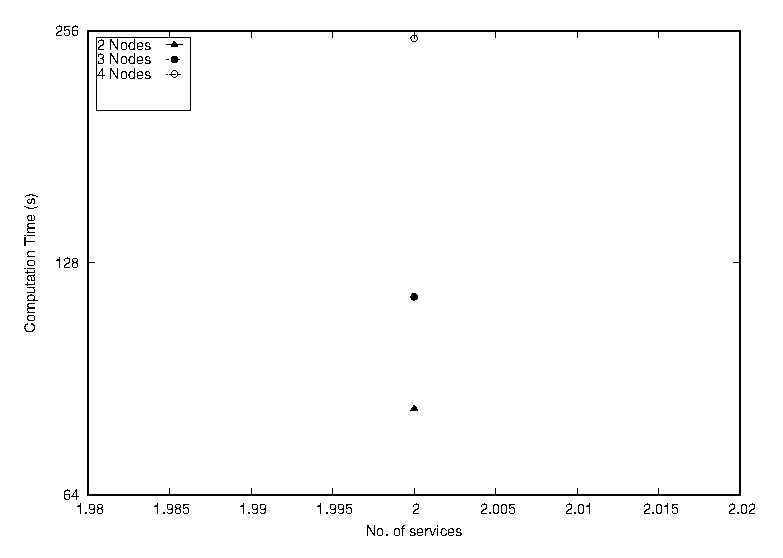
\includegraphics[width=0.95\columnwidth]{graphs/exhaustive_performance.eps}
  \caption{Exhaustive execution time evaluation. The x-axis represents the number of services, while the y-axis represents the execution time in seconds. The execution time is expressed both in linear and logarithmic scales.}
  \label{fig:perf_exhaustive}
\end{figure}

\begin{figure}[ht!]
  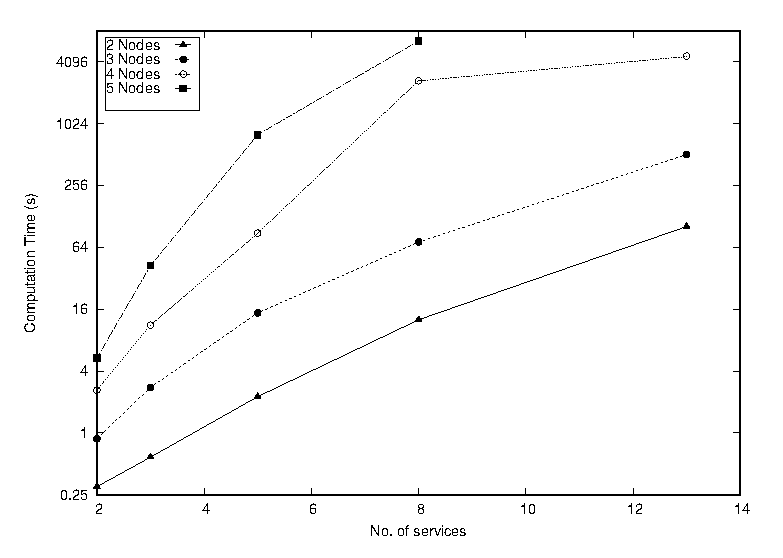
\includegraphics[width=0.95\columnwidth]{graphs/window_performance.eps}
  \caption{Preliminary performance evaluation.}
  \label{fig:perf_window}
\end{figure}


\begin{figure}[ht!]
  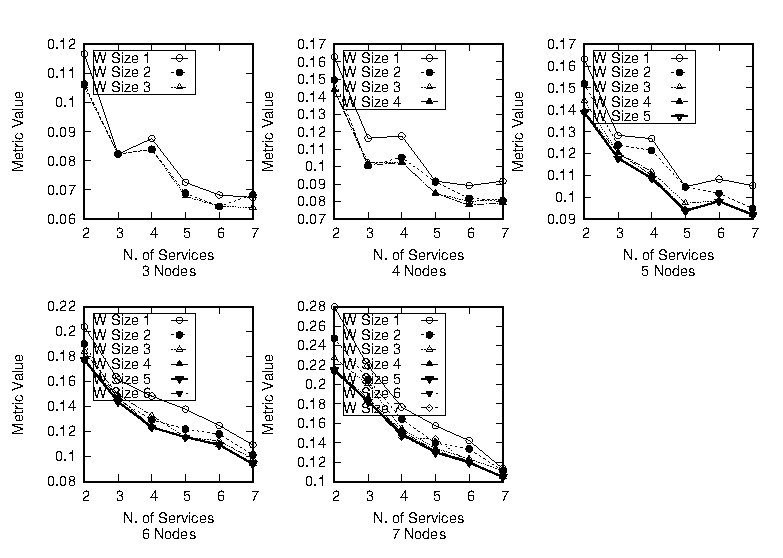
\includegraphics[width=0.95\columnwidth]{graphs/window_quality.eps}
  \caption{Quality evaluation.}
  \label{fig:quality_window}
\end{figure}

\usetikzlibrary{positioning}
\usetikzlibrary{backgrounds}



\begin{figure}[ht!]
  \centering
  \newcommand{\function}{$\instanceChartAnnotation{}$}
  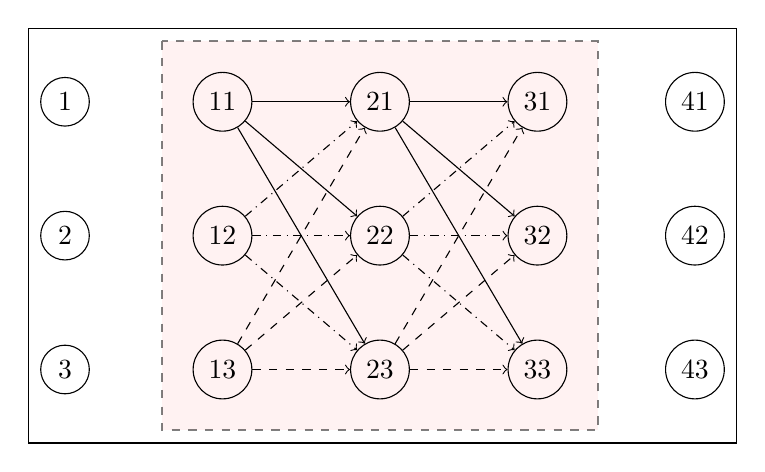
\begin{tikzpicture}[framed]
    \node[draw, circle] (s41) at (1,1.7) {$\sii{1}$};
    \node[draw, circle] (s42) at (1,0) {$\sii{2}$};
    \node[draw, circle] (s43) at (1,-1.7) {$\sii{3}$};

    \node[draw, circle] (s1) at (3,1.7) {$\sii{11}$};
    \node[draw, circle] (s2) at (3,0) {$\sii{12}$};
    \node[draw, circle] (s3) at (3,-1.7) {$\sii{13}$};

    \node[draw, circle] (s11) at (5,1.7) {$\sii{21}$};
    \node[draw, circle] (s12) at (5,0) {$\sii{22}$};
    \node[draw, circle] (s13) at (5,-1.7) {$\sii{23}$};

    \node[draw, circle] (s21) at (7,1.7) {$\sii{31}$};
    \node[draw, circle] (s22) at (7,0) {$\sii{32}$};
    \node[draw, circle] (s23) at (7,-1.7) {$\sii{33}$};

    \node[draw, circle] (s31) at (9,1.7) {$\sii{41}$};
    \node[draw, circle] (s32) at (9,0) {$\sii{42}$};
    \node[draw, circle] (s33) at (9,-1.7) {$\sii{43}$};


    % \draw[->] (node2) -- (node3);
    \draw[->] (s1) -- (s11);
    \draw[->] (s1) -- (s12);
    \draw[->] (s1) -- (s13);

    \draw[->,dashdotted] (s2) -- (s11);
    \draw[->,dashdotted] (s2) -- (s12);
    \draw[->,dashdotted] (s2) -- (s13);

    \draw[->,dashed] (s3) -- (s11);
    \draw[->,dashed] (s3) -- (s12);
    \draw[->,dashed] (s3) -- (s13);


    \draw[->] (s11) -- (s21);
    \draw[->] (s11) -- (s22);
    \draw[->] (s11) -- (s23);

    \draw[->,dashdotted] (s12) -- (s21);
    \draw[->,dashdotted] (s12) -- (s22);
    \draw[->,dashdotted] (s12) -- (s23);

    \draw[->,dashed] (s13) -- (s21);
    \draw[->,dashed] (s13) -- (s22);
    \draw[->,dashed] (s13) -- (s23);


    \begin{scope}[on background layer]
      \draw[thick, dashed, fill=red!10, opacity=0.5]
      ([shift={(-0.5,0.5)}]s1.north west) rectangle ([shift={(0.5,-0.5)}]s23.south east);

    \end{scope}
  \end{tikzpicture}
  \caption{Service composition instance}
  \label{fig:service_composition_instance}
\end{figure}
\subsection{Quality}
